\documentclass{article}

% Import packages
\usepackage{adjustbox}
\usepackage{amssymb}
\usepackage{amsmath}
\usepackage{amsthm}
\usepackage{appendix}
\usepackage{array}
\usepackage{bm}
\usepackage{booktabs}
\usepackage{caption}
\usepackage{colortbl}
\usepackage{epstopdf}
\usepackage{graphicx}
\usepackage[colorlinks=true, linkcolor=Brown, citecolor=DarkCyan, urlcolor=Olive]{hyperref}
\usepackage{lipsum}
\usepackage{mathtools}
\usepackage{multirow}
\usepackage[sort&compress, square, numbers]{natbib}
\usepackage[flushleft]{threeparttable}
\usepackage{url}
\usepackage[svgnames]{xcolor}

% Theorems-like enviroments
\newtheorem{assertion}{Assertion}
\newtheorem{assumption}{Assumption}
\newtheorem{conclusion}{Conclusion}
\newtheorem{corollary}{Corollary}
\newtheorem{definition}{Definition}
\newtheorem{example}{Example}
\newtheorem{lemma}{Lemma}
\newtheorem{proposition}{Proposition}
\newtheorem{remark}{Remark}
\newtheorem{result}{Result}
\newtheorem{theorem}{Theorem}

% Declare norms and absolute value
% http://tex.stackexchange.com/a/43009/62694
\DeclarePairedDelimiter\abs{\lvert}{\rvert}%
\DeclarePairedDelimiter\norm{\lVert}{\rVert}%
% Swap the definition of \abs* and \norm*, so that \abs and \norm resizes the size of the brackets, and the starred version does not.
\makeatletter
\let\oldabs\abs
\def\abs{\@ifstar{\oldabs}{\oldabs*}}
%
\let\oldnorm\norm
\def\norm{\@ifstar{\oldnorm}{\oldnorm*}}
\makeatother

% Triple norm
% https://tex.stackexchange.com/a/54392
\newcommand{\tnorm}[1]{{\left\vert\kern-0.25ex\left\vert\kern-0.25ex\left\vert #1\right\vert\kern-0.25ex\right\vert\kern-0.25ex\right\vert}}

% Generate links from DOIs
\newcommand*{\doi}[1]{\href{http://dx.doi.org/#1}{doi: #1}}

% Use the following commands to provide colored comments. Adapt according to the name of the authors.
\newcommand{\fa}[1]{\textcolor{magenta}{FA:~#1}} \newcommand{\sa}[1]{\textcolor{blue}{SA:~#1}}
\newcommand{\ta}[1]{\textcolor{orange}{TA:~#1}}

% You can add your custom commands here
\newcommand{\vecu}{\bm{u}}

% Title
\title{Name of the manuscript}
\author{First Author\footnote{Corresponding author e-mail: \href{mailto:first.author@institution.domain}{first.author@institution.domain}} $^{,}$\footnote{Department, Faculty, University, Country.} \and Second Author$^{\dagger}$ \and Third Author\footnote{Department, Faculty, University, Country.}}
\date{\today}

\begin{document}

% Title page
\maketitle
\begin{abstract}
\thispagestyle{empty}
\lipsum[1] \vspace{3mm} \\
\textbf{Keywords}: first keyword, second keyword, third keyword \vspace{3mm} \\
\textbf{Classification}: XXX, XXX, XXX \\
\end{abstract}
\newpage

% Highlights and TOC
\thispagestyle{empty}
\section*{Highlights}
\begin{itemize}
    \item First highlight.
    \item Second highlight.
    \item Third highlight.
\end{itemize}

\tableofcontents
\newpage

% Main body of the manuscript

\section{Introduction\label{sec:intro}}

While you are working on the manuscripts, authors can include colored comments. \fa{I'm the first author}. \sa{I'm the second author}. \ta{And I'm the third author}.

You can cite references in the usual way \cite{keilegavlen2021porepy}. Note that you can also group several references \cite{vohralik2005Poincare, pencheva2013mortar, repin2000variational}. If a reference contain a valid \texttt{DOI}, a link will be automatically be generated.

Figures are added in the usual way, see the code for Figure~\ref{fig:md_geo}. You can create beautiful tables such as Table~\ref{tab:errors}, using the \texttt{booktabs} package.

\begin{figure}[t]
    \centering
    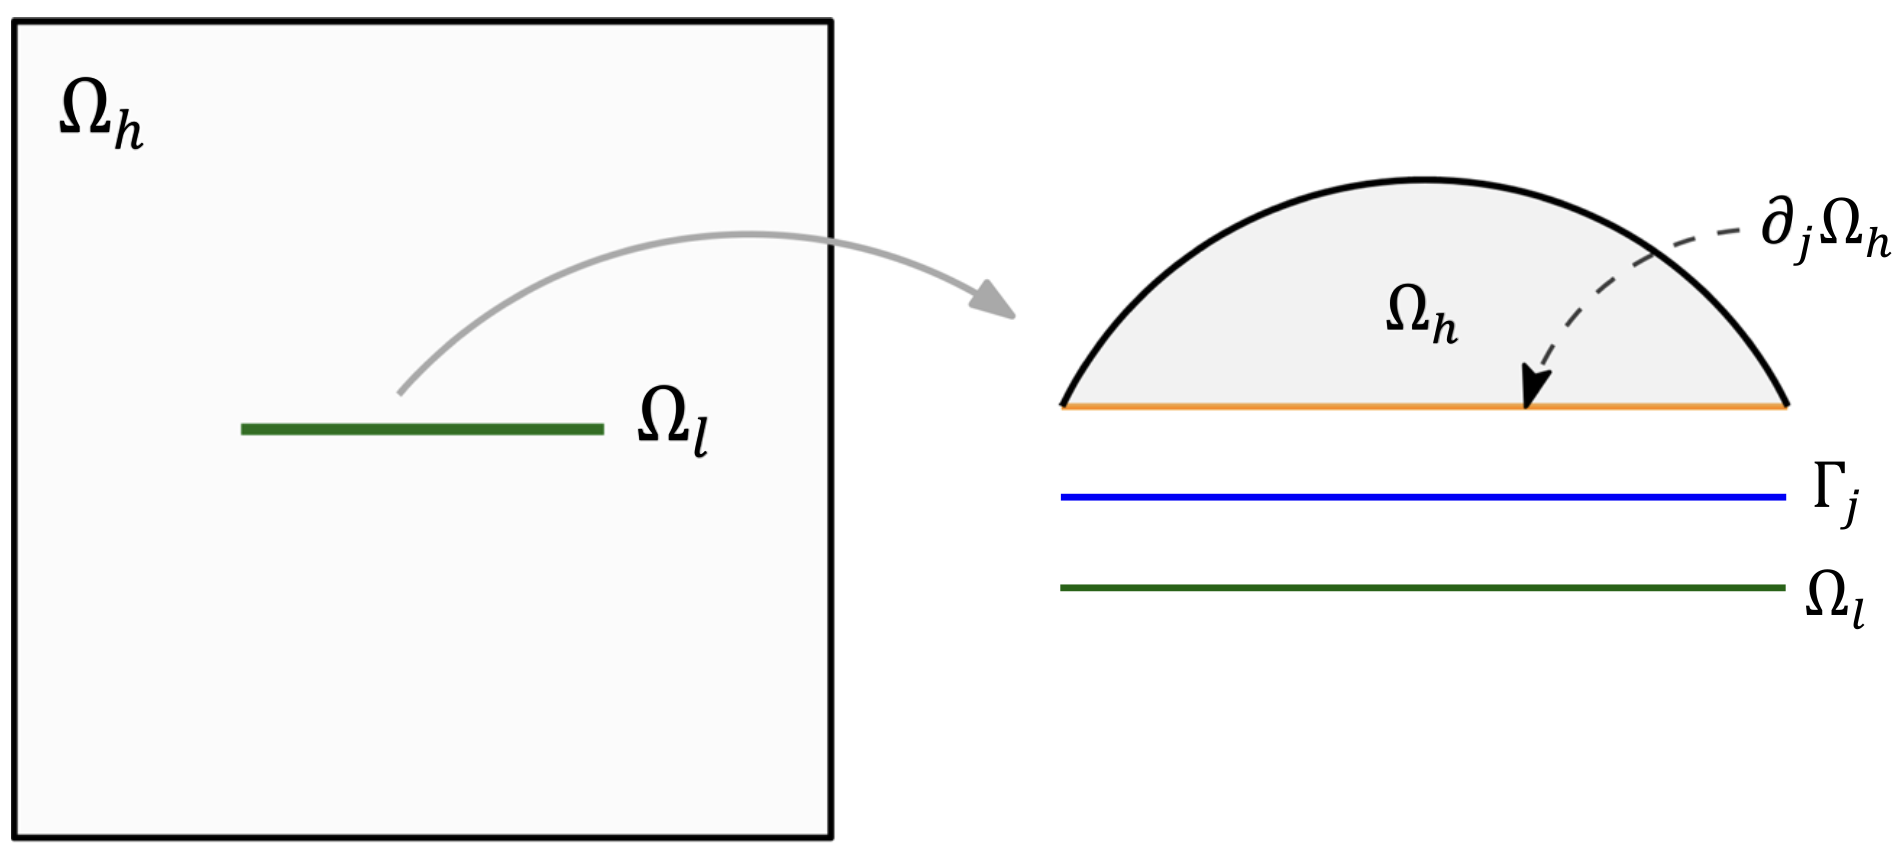
\includegraphics[width=0.75\textwidth]{fig_mixdim.png}
    \caption{Mixed-dimensional decomposition of a domain. Retrieved from \cite{keilegavlen2021porepy} under Creative Commons License. \label{fig:md_geo}}
\end{figure}

\begin{table}[t]
    \centering
    \caption{$L^2$-errors for several discretization techniques.\label{tab:errors}}
    \begin{tabular}{c c c}
         \textbf{Method} & \textbf{Error} & \textbf{Order} \\
         \toprule
         TPFA & $2.0\times10^{-3}$ & $2$ \\
         \midrule
         MPFA & $1.0\times10^{-3}$ & $2$ \\         \midrule
         CG-P1 & $1.5\times10^{-3}$ & $2$ \\
         \midrule
         RT0-P0 & $1.1\times10^{-3}$ & $2$ \\
         \bottomrule
    \end{tabular}
\end{table}

\section{Second section\label{sec:second_sec}}

Operators for absolute value $\abs{x}$, norm $\norm{p}$, and triple norm $\tnorm{\vecu}$ are readily available.

\section{Third section\label{sec:third_sec}}

Several environments for writing theorems and similar are included for convenience. For instance, \textit{theorem}, \textit{corollary}, \textit{proposition}, \textit{lemma}, \textit{assertion}, \textit{result}, \textit{conclusion}, \textit{definition}, \textit{assumption}, \textit{example}, and \textit{remark}. You can always create a custom one using \texttt{$\backslash$newtheorem\{\}}.

\begin{theorem}[A new amazing theorem.]
    Let $x=a$ and $y=b$. Then, $x + y = a + b$.
\end{theorem}

\begin{proof}
    The proof is left to the reader.
\end{proof}


\section{Conclusion\label{sec:conclusion}}

A difficult to write conclusion goes here.

\section*{Acknowledgments}

Funding and acknowledgments go here.

% Bibliography
\bibliographystyle{unsrtnat}
\bibliography{refs.bib}

% Appendices
\begin{appendices}
\section{First appendix\label{sec:first_appx}}
An appendix can be added here.
\section{Second appendix\label{sec:second_appx}}
You can have several appendices if you want.
\end{appendices}

\end{document}
